\section{弱收敛的定义}
\label{sec:weak-definition}

设$P_1,P_2,\dots$与$P$都是$\mathbb{R}^{d}$上的概率分布，即Borel集族$\mathcal{B}(\mathbb{R}^{d})$上的概率测度。我们要给“$P_n$趋近$P$”一个确切的含义，它只用到这些分布，与产生它们的样本空间无关。先用观测函数的平均作比较，得到定义；再把它与第~\ref{chap:random-variable-convergence}章在共同样本空间上的依概率收敛作对照。

\subsection{分布与测试函数}
\label{sec:weak-test-functions}

比较两个分布，一个直接的办法是选定一个观测函数$f$，看两个分布下$f$的平均
\[
 \int f\,\mathrm{d}P_n\quad\text{与}\quad\int f\,\mathrm{d}P .
\]
把分布看成总量为一的质量，$\int f\,\mathrm{d}P$就是用$f$加权后的总质量。若$f$是某个区间的示性函数，读数就是落在区间里的质量，直方图的每一根柱正是这样一次读数。如果对足够多的$f$读数都接近，就可以说两个分布接近。

问题在于选哪些$f$。第一个要求是有界。对有界的$f$，任何概率分布下的平均都有定义，并且读数的绝对值不超过$\sup\lvert f\rvert$。若允许无界的$f$，例如$f(x)=x$，有的分布（如第~\ref{chap:common-distributions}章的Cauchy分布）根本没有这个平均；第~\ref{sec:weak-integral-limits}节还会看到，极少的质量跑到远处，就能让无界函数的读数变化很大。

第二个要求是连续。设$P_n$是集中在$1/n$的单点分布，$P$集中在$0$。两个质点的位置只差$1/n$，我们希望说$P_n$趋近$P$。若用$f=\mathbf{1}_{(0,\infty)}$读数，$P_n$下的平均恒为$1$，$P$下却是$0$。示性函数在$0$处跳跃，把“稍偏右”与“恰在$0$”截然分开。连续函数对位置的微小变动只给出微小变化：
\[
 \int f\,\mathrm{d}P_n=f(1/n)\longrightarrow f(0)=\int f\,\mathrm{d}P .
\]

把$\mathbb{R}^{d}$上全体有界连续实函数记作$C_b(\mathbb{R}^{d})$。按上面两条要求，用它们作为比较分布的读数。

\begin{definition}[弱收敛与依分布收敛]
\label{def:weak-convergence}
设$P_n$（$n\geq1$）与$P$是$\mathbb{R}^{d}$上的概率分布。若对每个$f\in C_b(\mathbb{R}^{d})$，
\begin{equation}
 \lim_{n\to\infty}\int f\,\mathrm{d}P_n=\int f\,\mathrm{d}P ,
 \label{eq:weak-definition}
\end{equation}
则称$P_n$\term{弱收敛}（weak convergence）到$P$，记作$P_n\xrightarrow{\mathrm{w}}P$。设随机向量$\bm{X}_n$定义在概率空间$(\Omega_n,\mathcal{F}_n,\mathbb{P}_n)$上，$\bm{X}$定义在$(\Omega,\mathcal{F},\mathbb{P})$上。若$P_{\bm{X}_n}\xrightarrow{\mathrm{w}}P_{\bm{X}}$，即对每个$f\in C_b(\mathbb{R}^{d})$都有
\begin{equation}
 \lim_{n\to\infty}\mathbb{E}\bigl[f(\bm{X}_n)\bigr]=\mathbb{E}\bigl[f(\bm{X})\bigr] ,
 \label{eq:weak-convergence-in-distribution}
\end{equation}
则称$\bm{X}_n$\term{依分布收敛}（convergence in distribution）到$\bm{X}$，记作$\bm{X}_n\xrightarrow{\mathrm{d}}\bm{X}$，也写作$\bm{X}_n\xrightarrow{\mathrm{d}}P_{\bm{X}}$。
\end{definition}

式~\eqref{eq:weak-convergence-in-distribution}左边的期望在$\Omega_n$上计算，为简洁不写下标。$f$叫作\term{测试函数}（test function）。这个定义的要点是：$\bm{X}_n$与$\bm{X}$可以定义在不同的样本空间上，比较只通过它们的分布进行。“随机变量依分布收敛”只是“分布弱收敛”的另一种说法，它不断言$\bm{X}_n$的取值与$\bm{X}$的取值越来越近，因为$\bm{X}_n-\bm{X}$可能根本没有定义。

\paragraph{格点上的均匀分布}
回到章首的$U_n$。对$f\in C_b(\mathbb{R})$，
\[
 \mathbb{E}\bigl[f(U_n)\bigr]=\frac1n\sum_{k=1}^{n}f\Bigl(\frac kn\Bigr) .
\]
这正是$f$在$[0,1]$上取右端点的Riemann和。$f$在$[0,1]$上连续，因而可积，Riemann和收敛到积分（可参考\BookChapterRef{chap:univariate-integration}{卷一第7章“一元函数的积分”}）。设$U\sim\operatorname{Unif}(0,1)$，于是
\[
 \lim_{n\to\infty}\mathbb{E}\bigl[f(U_n)\bigr]=\int_0^1f(x)\,\mathrm{d}x=\mathbb{E}\bigl[f(U)\bigr] ,
\]
即$U_n\xrightarrow{\mathrm{d}}\operatorname{Unif}(0,1)$。

取一个具体的测试函数$f(x)=\min(x^2,1)$，它在$[0,1]$上就是$x^2$。由平方和公式，
\[
 \mathbb{E}\bigl[f(U_n)\bigr]=\frac{1}{n^{3}}\sum_{k=1}^{n}k^{2}=\frac{(n+1)(2n+1)}{6n^{2}} .
\]
$n=5,10,50$时依次为
\[
 0.4400,\qquad 0.3850,\qquad 0.3434,
\]
逐渐接近$\int_0^1x^2\,\mathrm{d}x=1/3$。图~\ref{fig:weak-lattice-uniform}(a)中，柱的面积之和就是这个读数；(b)画出读数随$n$的变化。每个格点的质量$1/n$趋于零，读数却收敛：弱收敛比较的是质量的整体摆放，而不是单点的质量。

\begin{BookInlineFigure}
 \centering
 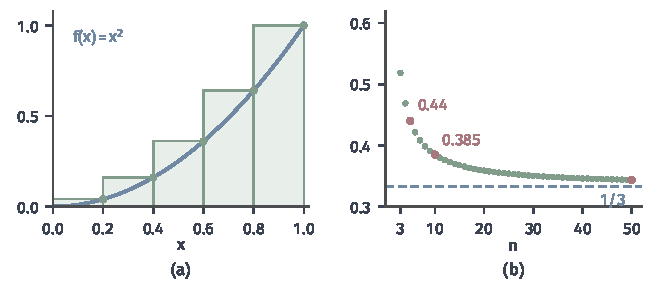
\includegraphics[width=112mm]{figures/07-probability/03-probability-limits/matplotlib/weak-lattice-uniform/figure.pdf}
 \caption{格点均匀分布的弱收敛。(a)$n=5$，浅绿柱宽$1/5$、高$f(k/5)$（绿点），面积之和为$\mathbb{E}[f(U_5)]=0.44$；蓝线为测试函数$f(x)=x^2$，其下面积为$1/3$。(b)$\mathbb{E}[f(U_n)]$随$n$的变化（绿点），蓝色虚线为极限$1/3$。}
 \label{fig:weak-lattice-uniform}
\end{BookInlineFigure}

\paragraph{极限的唯一性}
一列数的极限唯一。对分布也应如此，否则“极限分布”就不是一个确定的对象。这归结为：有界连续函数的读数能否区分两个分布。下面构造一族连续函数，从上方逼近闭集的示性函数。

对闭集$F\subset\mathbb{R}^{d}$，记点$\bm{x}$到$F$的距离为
\[
 \operatorname{dist}(\bm{x},F)=\inf_{\bm{y}\in F}\lVert\bm{x}-\bm{y}\rVert_2 ,
\]
并令
\begin{equation}
 f_k(\bm{x})=\max\bigl(0,\,1-k\operatorname{dist}(\bm{x},F)\bigr),\qquad k=1,2,\dots .
 \label{eq:weak-closed-approx}
\end{equation}
由三角不等式，距离函数满足
\[
 \lvert\operatorname{dist}(\bm{x},F)-\operatorname{dist}(\bm{y},F)\rvert\leq\lVert\bm{x}-\bm{y}\rVert_2 ,
\]
所以$f_k$连续，并且是Lipschitz常数为$k$的Lipschitz函数。它在$F$上等于$1$，在距$F$不小于$1/k$处等于$0$，取值在$[0,1]$中。

\begin{lemma}[有界连续函数确定分布]
\label{lem:weak-uniqueness}
设$P,Q$是$\mathbb{R}^{d}$上的概率分布。若对每个$f\in C_b(\mathbb{R}^{d})$都有$\int f\,\mathrm{d}P=\int f\,\mathrm{d}Q$，则$P=Q$。因此弱收敛的极限唯一：若$P_n\xrightarrow{\mathrm{w}}P$且$P_n\xrightarrow{\mathrm{w}}Q$，则$P=Q$。
\end{lemma}

\begin{proof}
取闭集$F$与式~\eqref{eq:weak-closed-approx}中的$f_k$。若$\bm{x}\in F$，则$f_k(\bm{x})=1$。若$\bm{x}\notin F$，因$F$闭，$\operatorname{dist}(\bm{x},F)>0$，当$k>1/\operatorname{dist}(\bm{x},F)$时$f_k(\bm{x})=0$。所以$f_k$逐点不增地趋于$\mathbf{1}_F$。

$0\leq f_k\leq1$，由支配收敛定理，
\[
 P(F)=\lim_{k\to\infty}\int f_k\,\mathrm{d}P=\lim_{k\to\infty}\int f_k\,\mathrm{d}Q=Q(F) .
\]
于是$P$与$Q$在全体闭集上相等。闭集族对有限交封闭，并且生成$\mathcal{B}(\mathbb{R}^{d})$。由第~\ref{chap:probability-spaces}章测度的唯一性定理，$P=Q$。

若$P_n$同时弱收敛到$P$和$Q$，则对每个$f\in C_b(\mathbb{R}^{d})$，$\int f\,\mathrm{d}P$与$\int f\,\mathrm{d}Q$是同一数列的极限，二者相等，再由前半部分得$P=Q$。
\end{proof}

\paragraph{同分布而样本不接近}
依分布收敛不涉及样本，下面的例子把这一点推到极端。取$\Omega=[0,1]$，$\mathbb{P}$为长度，令
\[
 X(\omega)=\omega,\qquad Y(\omega)=1-\omega .
\]
对$0\leq x\leq1$，$\mathbb{P}(Y\leq x)=\mathbb{P}(\omega\geq1-x)=x$，所以$X$与$Y$都服从$\operatorname{Unif}(0,1)$。令$X_n=Y$对一切$n$成立，则$X_n$与$X$的分布完全相同，$X_n\xrightarrow{\mathrm{d}}X$平凡地成立。

可是在样本点$\omega$上，$X_n$与$X$相差$\lvert1-2\omega\rvert$，与$n$无关，并且
\[
 \mathbb{P}\bigl(\lvert X_n-X\rvert>1/2\bigr)=\mathbb{P}\bigl(\omega<1/4\text{ 或 }\omega>3/4\bigr)=\frac12 .
\]
图~\ref{fig:weak-same-law}(a)画出这两个$\Omega$上的函数，它们在大部分样本点上相距很远；(b)是它们的直方图，完全一样。这好比两个班的身高分布相同，并不意味着按学号配对的两人身高接近。依分布收敛只比较“分布”这一侧，不管它由哪个函数实现。

\begin{BookInlineFigure}
 \centering
 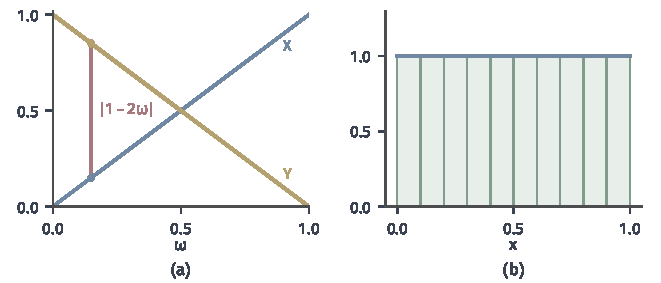
\includegraphics[width=112mm]{figures/07-probability/03-probability-limits/matplotlib/weak-same-law/figure.pdf}
 \caption{同分布而样本不接近。(a)$\Omega=[0,1]$上的$X(\omega)=\omega$（蓝）与$Y(\omega)=1-\omega$（黄），红色竖线段标出一个样本点上的差$\lvert1-2\omega\rvert$。(b)二者各用$\omega$的$2000$个等距点算出的直方图（浅绿），与$\operatorname{Unif}(0,1)$的密度（蓝）一致。}
 \label{fig:weak-same-law}
\end{BookInlineFigure}

\subsection{与依概率收敛的关系}
\label{sec:weak-probability-convergence}

当$\bm{X}_n$与$\bm{X}$定义在同一概率空间上时，第~\ref{chap:random-variable-convergence}章的依概率收敛$\bm{X}_n\xrightarrow{\mathbb{P}}\bm{X}$也有意义：对每个$\varepsilon>0$，事件$\lVert\bm{X}_n-\bm{X}\rVert_2\geq\varepsilon$的概率趋于零。上一个例子说明依分布收敛不能推出依概率收敛。反方向则成立：样本接近时，分布也接近。

\begin{theorem}[依概率收敛蕴含依分布收敛]
\label{thm:weak-prob-implies-dist}
设$\bm{X}_n$与$\bm{X}$是同一概率空间上取值于$\mathbb{R}^{d}$的随机向量。若$\bm{X}_n\xrightarrow{\mathbb{P}}\bm{X}$，则$\bm{X}_n\xrightarrow{\mathrm{d}}\bm{X}$。
\end{theorem}

\begin{proof}
取$f\in C_b(\mathbb{R}^{d})$，记$M=\sup\lvert f\rvert$，任取$\varepsilon>0$。困难在于$f$在整个空间上未必一致连续，所以先把$\bm{X}$限制在一个有界范围内。事件$\{\lVert\bm{X}\rVert_2>r\}$随$r$增大而下降到空集，由概率的连续性，存在$r$使$\mathbb{P}(\lVert\bm{X}\rVert_2>r)<\varepsilon$。

闭球$B=\{\lVert\bm{x}\rVert_2\leq r+1\}$是紧集，$f$在$B$上一致连续。于是存在$\delta\in(0,1)$，使得$\bm{x},\bm{y}\in B$且$\lVert\bm{x}-\bm{y}\rVert_2<\delta$时$\lvert f(\bm{x})-f(\bm{y})\rvert<\varepsilon$。

若$\lVert\bm{X}\rVert_2\leq r$且$\lVert\bm{X}_n-\bm{X}\rVert_2<\delta$，则$\bm{X}$与$\bm{X}_n$都在$B$中，$\lvert f(\bm{X}_n)-f(\bm{X})\rvert<\varepsilon$。其余情形用$\lvert f(\bm{X}_n)-f(\bm{X})\rvert\leq2M$。两部分合起来，
\[
 \bigl\lvert\mathbb{E}[f(\bm{X}_n)]-\mathbb{E}[f(\bm{X})]\bigr\rvert
 \leq\varepsilon+2M\,\mathbb{P}\bigl(\lVert\bm{X}\rVert_2>r\bigr)+2M\,\mathbb{P}\bigl(\lVert\bm{X}_n-\bm{X}\rVert_2\geq\delta\bigr) .
\]
令$n\to\infty$，最后一项趋于零，所以
\[
 \limsup_{n\to\infty}\bigl\lvert\mathbb{E}[f(\bm{X}_n)]-\mathbb{E}[f(\bm{X})]\bigr\rvert\leq\varepsilon+2M\varepsilon .
\]
$\varepsilon$任意，左边为零。
\end{proof}

反方向不成立，离散的例子更直接。设$X\sim\operatorname{Bern}(1/2)$，令$X_n=1-X$。$X_n$也服从$\operatorname{Bern}(1/2)$，所以$X_n\xrightarrow{\mathrm{d}}X$；但$\lvert X_n-X\rvert=1$恒成立，$\mathbb{P}(\lvert X_n-X\rvert\geq1/2)=1$。

\paragraph{极限为常量}
有一种情形反向结论成立：极限分布集中在一个点$\bm{c}$上。常量在任何概率空间上都可以定义，$\bm{X}_n\xrightarrow{\mathbb{P}}\bm{c}$只要求事件$\lVert\bm{X}_n-\bm{c}\rVert_2\geq\varepsilon$的概率趋于零，其中的概率在$\bm{X}_n$所在的空间上计算，所以即使各$\bm{X}_n$在不同的空间上，这个说法也有意义。

\begin{theorem}[依分布趋于常量]
\label{thm:weak-constant-limit}
设$\bm{c}\in\mathbb{R}^{d}$。若$\bm{X}_n\xrightarrow{\mathrm{d}}\bm{c}$，则对每个$\varepsilon>0$，
\begin{equation}
 \lim_{n\to\infty}\mathbb{P}\bigl(\lVert\bm{X}_n-\bm{c}\rVert_2\geq\varepsilon\bigr)=0 ,
 \label{eq:weak-constant-limit}
\end{equation}
即$\bm{X}_n\xrightarrow{\mathbb{P}}\bm{c}$。
\end{theorem}

\begin{proof}
令
\[
 h(\bm{x})=\min\bigl(1,\lVert\bm{x}-\bm{c}\rVert_2/\varepsilon\bigr) .
\]
它有界连续，$h(\bm{c})=0$，并且在$\lVert\bm{x}-\bm{c}\rVert_2\geq\varepsilon$处等于$1$，所以$h$处处不小于偏离事件$\{\lVert\bm{x}-\bm{c}\rVert_2\geq\varepsilon\}$的示性函数。取期望，
\[
 \mathbb{P}\bigl(\lVert\bm{X}_n-\bm{c}\rVert_2\geq\varepsilon\bigr)\leq\mathbb{E}\bigl[h(\bm{X}_n)\bigr]\longrightarrow h(\bm{c})=0 .
\]
\end{proof}

证明用一个连续函数从上方压住“偏离$\bm{c}$至少$\varepsilon$”的示性函数，见图~\ref{fig:weak-constant-limit}。常量之所以特殊，是因为它没有随机性需要与$\bm{X}_n$配对：知道$\bm{X}_n$的分布集中到$\bm{c}$附近，就知道$\bm{X}_n$本身以大概率在$\bm{c}$附近。第~\ref{sec:weak-slutsky}节的Slutsky定理要用到这一点。

\begin{BookInlineFigure}
 \centering
 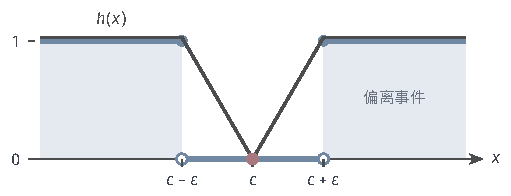
\includegraphics[width=86.6mm]{figures/07-probability/03-probability-limits/tikz/weak-constant-limit/figure.pdf}
 \caption{常量极限的证明。深灰折线为$h(x)=\min(1,\lvert x-c\rvert/\varepsilon)$，它连续且在$c$处为零；浅蓝区域为偏离事件$\{\lvert x-c\rvert\geq\varepsilon\}$，其示性函数（蓝色粗线）处处不超过$h$。}
 \label{fig:weak-constant-limit}
\end{BookInlineFigure}
